Le LMUL est un nombre pouvant prendre les valeurs : \texttt{1/8, 1/4, 1/2, 1, 2, 4} ou \texttt{8}. Il fait partie intégrante de la configuration d'un registre vectoriel dans le language assembleur, c'est à dire que le nombre d'éléments dans un tel registre dépend seulement de 3 choses: 
\begin{itemize}
	\item La taille des registres vectoriels simple (déterminée par le matériel).
	\item Le type des éléments contenu dans le vecteur.
	\item La valeur du LMUL.
\end{itemize}

Sa fonctionnalité quand il est inférieur à 1 est légèrement différente par rapport aux autres valeurs, mais sa logique reste la même.

\subsubsection{LMUL>=1}

Lorsque le LMUL est supérieur ou égal à 1, sa valeur désigne le nombre de registres vectoriels groupés qui vont former le vecteur final. Soit SEW le nombre de bits sur lequel est matériellement codé un registre vectoriel, au bas niveau, lors de la configuration d'un registre vectoriel en assembleur, au lieu de réserver SEW bits, la machine va réserver $SEW\times LMUL$ bits pour le vecteur. C'est à dire que tous les registres vectoriels matériels groupés doivent être placés sur une mémoire contigüe. Ainsi, les registres vectoriels des jeux d'instructions plus classiques sont des registres vectoriels configuré avec LMUL=1. Un exemple avec LMUL=2 est illustré en figure \ref{fig:LMUL}, où les r$i$, $i\in \{0, nombreRegistresVectoriels-1\}$ représentent les registres vectoriels matériels.\\


\begin{figure}[H]
    \centering
    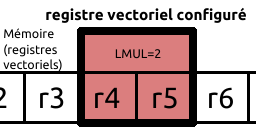
\includegraphics[width=0.4\linewidth]{img/LMUL.png}
    \caption{Exemple avec LMUL=2}
    \label{fig:LMUL}
\end{figure}


Cette fonctionnalité trouve son utilité dans l'optimisation de performances. En effet, une fois qu'un registre vectoriel est configuré avec un LMUL>1, effectuer une opération sur ce vecteur ne prendra qu'une seule instruction assembleur, ce qui permet de vectoriser jusqu'à 8 fois plus de données qu'une vectorisation classique. 



\subsubsection{LMUL<1}

Puis, quand le LMUL est inférieur à 1, au lieu de grouper des vecteurs, il divise le vecteur: en configurant le registre vectoriel avec LMUL = 1/2, il n'y a que la moitié du registre vectoriel matériel qui est utilisée pour remplir les données et faire les opérations.\\

Le nombre d'applications de cette fonctionnalité étant relativement restreint, elle n'a pas été inclue à MIPP, il n'est possible que d'utiliser des LMUL supérieurs ou égaux à 1.